% ===========================================================================
% Reusable TikZ / pgfplots figure macros.
%
% Every figure in this thesis is generated here from the CSV files in data/,
% which are exported directly from rust_metrics/results/. No number in any
% figure is typed by hand.
% ===========================================================================

\usetikzlibrary{arrows.meta, positioning, fit, backgrounds, calc, shapes.geometric, patterns}
\pgfplotsset{compat=1.18}

% ---------------------------------------------------------------- house style
% TUM blue for diagrams and single-series charts; Okabe-Ito hues for series
% that stand for a snapshot, matching the dashboard so a snapshot keeps its
% colour between screen and page.
\definecolor{kgblue}{HTML}{3070B3}   % TUM blue: diagrams, single series
\definecolor{kgnavy}{HTML}{072140}   % TUM dark blue
\definecolor{kgamber}{HTML}{E69F00}  % yago-4
\definecolor{kggreen}{HTML}{009E73}  % yago-4.5.0.2
\definecolor{kgviolet}{HTML}{CC79A7} % dbpedia-2015
\definecolor{kgolive}{HTML}{7F6F00}  % dbpedia-2025
\definecolor{kgred}{HTML}{D55E00}    % emphasis: cut lines, rings
\definecolor{kgteal}{HTML}{0072B2}
\definecolor{kggrey}{HTML}{6B7280}
\definecolor{kgpale}{HTML}{EAF1F8}
\definecolor{kgpale2}{HTML}{F4F6FA}

\pgfplotsset{
  kgaxis/.style={
    width=\linewidth,
    font=\footnotesize,
    axis line style={kggrey!60},
    tick align=outside,
    tick style={kggrey!60},
    grid=major,
    grid style={kggrey!25, dashed},
    legend style={draw=kggrey!40, fill=white, font=\scriptsize,
                  cells={anchor=west}},
    every axis title/.append style={font=\small\bfseries},
    % one swatch per legend entry; the bar-plot default draws two
    area legend,
  },
  kgbar/.style={
    kgaxis,
    xbar,
    bar width=5pt,
    y=13pt,
    enlarge y limits=0.12,
    xmin=0,
    nodes near coords,
    every node near coord/.append style={font=\tiny, color=black!75,
      /pgf/number format/fixed, /pgf/number format/precision=2},
    ytick=data,
    yticklabel style={font=\scriptsize},
  },
}

% dbpedia-2016 and 2022 colours, from the dashboard palette
\definecolor{kgorange}{HTML}{D55E00}  % dbpedia-2016
\definecolor{kgsky}{HTML}{56B4E9}     % dbpedia-2022

% Cross-graph entropy gap per class, one marker per DBpedia release. Used for
% Tables 4.10 and 4.11; #1 = CSV, #2 = panel title, #3 = axis height.
\newcommand{\figgapdots}[3]{%
  \begin{axis}[
    kgaxis, scale only axis, width=3.7cm, height=#3,
    title={#2},
    y dir=reverse, ytick=data,
    table/col sep=comma,
    yticklabels from table={#1}{class},
    yticklabel style={font=\scriptsize},
    xmin=0, xmax=9.2, xtick={0,2,4,6,8},
    xlabel={$|H_{\text{YAGO}} - H_{\text{DBpedia}}|$ (bits)},
    xmajorgrids=true, ymajorgrids=true,
    enlarge y limits=0.04,
    % marks only: draw one marker as the legend swatch, not the area default
    legend image code/.code={\draw[mark repeat=2, mark phase=2, ##1]
      plot coordinates {(0cm,0cm) (0.2cm,0cm) (0.4cm,0cm)};},
    legend columns=2,
    legend style={at={(rel axis cs:0.5,0)}, anchor=north, yshift=-30pt,
                  /tikz/every even column/.append style={column sep=6pt}},
  ]
    \addplot[only marks, mark=*, mark size=2pt, color=kgviolet]
      table[col sep=comma, x=gap2015, y expr=\coordindex]{#1};
    \addplot[only marks, mark=square*, mark size=1.8pt, color=kgorange]
      table[col sep=comma, x=gap2016, y expr=\coordindex]{#1};
    \addplot[only marks, mark=triangle*, mark size=2.3pt, color=kgsky]
      table[col sep=comma, x=gap2022, y expr=\coordindex]{#1};
    \addplot[only marks, mark=diamond*, mark size=2.4pt, color=kgolive]
      table[col sep=comma, x=gap2025, y expr=\coordindex]{#1};
    \legend{2015, 2016, 2022, 2025}
  \end{axis}%
}

\tikzset{
  stage/.style={
    draw=kgblue!70, fill=kgpale, line width=.6pt, rounded corners=2pt,
    align=center, font=\footnotesize, inner sep=5pt, minimum height=9mm,
    text width=23mm},
  store/.style={
    draw=kggrey!70, fill=kgpale2, line width=.6pt, align=center,
    font=\footnotesize, inner sep=5pt, minimum height=9mm, text width=23mm},
  note/.style={font=\scriptsize\itshape, color=kggrey, align=center},
  flow/.style={-{Stealth[length=5pt]}, draw=kggrey, line width=.6pt},
  flowback/.style={{Stealth[length=5pt]}-{Stealth[length=5pt]}, draw=kggrey,
                   line width=.6pt, dashed},
}

% ===========================================================================
% Figure: the measurement pipeline (Chapter 3)
% Two lanes rather than one row: six stages in a line need ~204mm and the text
% block is 146mm. The split also carries the point of the figure, since the
% counting stays in the server lane and only counts cross into the client lane.
% ===========================================================================
\newcommand{\figpipeline}{%
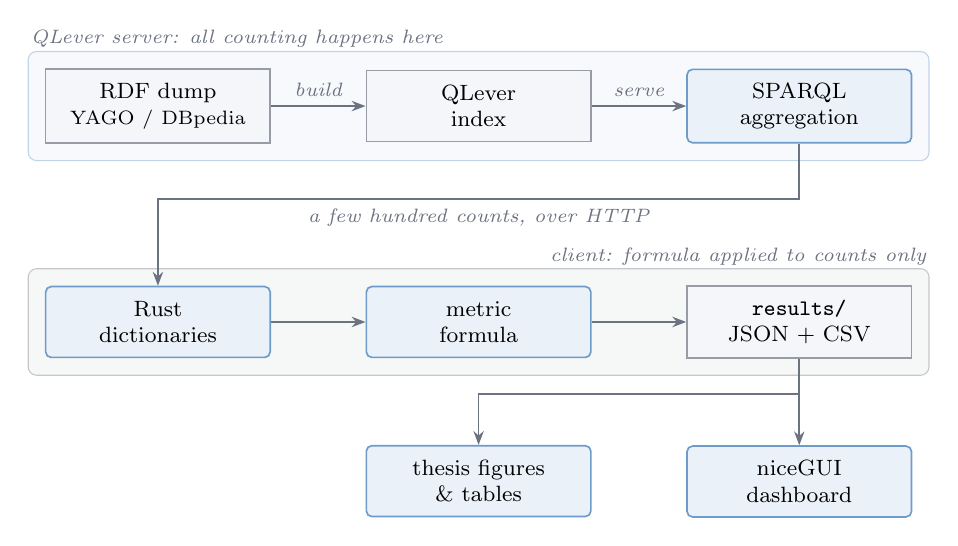
\begin{tikzpicture}[node distance=18mm and 12mm,
    pbox/.style={stage, text width=25mm},
    pstore/.style={store, text width=25mm}]
  % server lane
  \node[pstore]              (kg)     {RDF dump\\\scriptsize YAGO / DBpedia};
  \node[pstore, right=of kg] (index)  {QLever\\index};
  \node[pbox, right=of index](sparql) {SPARQL\\aggregation};
  % client lane
  \node[pbox, below=of kg]       (rust)    {Rust\\dictionaries};
  \node[pbox, right=of rust]     (formula) {metric\\formula};
  \node[pstore, right=of formula](json)    {\texttt{results/}\\JSON + CSV};
  % outputs
  \node[pbox, below=11mm of json]    (dash) {niceGUI\\dashboard};
  \node[pbox, below=11mm of formula] (figs) {thesis figures\\\& tables};

  \draw[flow] (kg) -- node[above, note] {build} (index);
  \draw[flow] (index) -- node[above, note] {serve} (sparql);
  \draw[flow] (sparql.south) -- ++(0,-7mm) -| (rust.north)
        node[pos=.25, below, note] {a few hundred counts, over HTTP};
  \draw[flow] (rust) -- (formula);
  \draw[flow] (formula) -- (json);
  \coordinate (fork) at ($(json.south)+(0,-4.5mm)$);
  \draw[draw=kggrey, line width=.6pt] (json.south) -- (fork);
  \draw[flow] (fork) -- (dash.north);
  \draw[flow] (fork) -| (figs.north);

  \begin{scope}[on background layer]
    \node[fit=(kg)(index)(sparql), draw=kgblue!30, fill=kgblue!4,
          rounded corners=3pt, inner sep=6pt] (server) {};
    \node[fit=(rust)(formula)(json), draw=kggrey!40, fill=kggrey!6,
          rounded corners=3pt, inner sep=6pt] (client) {};
  \end{scope}
  \node[note, anchor=south west, inner sep=1pt] at (server.north west)
       {QLever server: all counting happens here};
  \node[note, anchor=south east, inner sep=1pt] at (client.north east)
       {client: formula applied to counts only};
\end{tikzpicture}}

% ===========================================================================
% Figure: count-of-counts histogram (Chapter 3, efficiency)
% ===========================================================================
\newcommand{\fighistogram}{%
\begin{tikzpicture}
  \node[store, text width=30mm] (naive) {stream every object value\\\scriptsize $O(|T_t|)$ rows};
  \node[stage, right=26mm of naive, text width=30mm] (cc)
       {count-of-counts histogram\\\scriptsize $O(|\text{distinct counts}|)$ rows};
  \draw[flow] (naive) -- node[above, note] {nested} node[below, note] {\texttt{GROUP BY}} (cc);
  % notes share one baseline under the taller box, so they line up
  \coordinate (base) at ($(cc.south)+(0,-2mm)$);
  \node[note, anchor=north] at (naive.south |- base) {millions of rows cross the wire};
  \node[note, anchor=north] at (cc.south |- base) {a few hundred rows};
  \node[font=\footnotesize, anchor=north] (eq) at ($(naive.south |- base)!0.5!(cc.south |- base)+(0,-8mm)$)
       {$H = \log_2 N - \dfrac{1}{N}\displaystyle\sum_{c} m_c \cdot c \cdot \log_2 c$};
  \node[note, below=1mm of eq] {exact, not sampled: entropy depends only on the multiset of counts};
\end{tikzpicture}}

% ===========================================================================
% Figure: subject-window scoping (Chapter 3, metric 10)
% ===========================================================================
\newcommand{\figwindow}{%
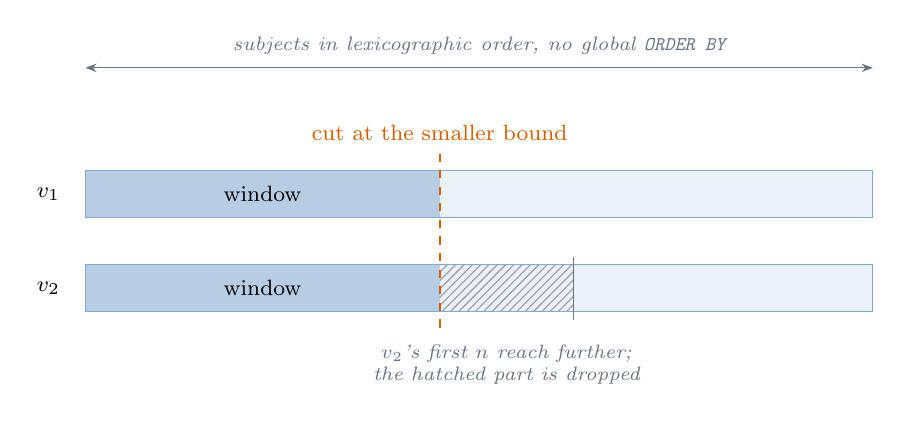
\begin{tikzpicture}[x=1mm, y=1mm, font=\footnotesize]
  % each version lists its subjects in lexicographic order; v1's first n end
  % earlier (x=45) than v2's (x=62), so both are cut at x=45
  \fill[kgpale]    (0,12) rectangle (100,18);
  \fill[kgblue!35] (0,12) rectangle (45,18);
  \draw[kgblue!60] (0,12) rectangle (100,18);
  \fill[kgpale]    (0,0) rectangle (100,6);
  \fill[kgblue!35] (0,0) rectangle (45,6);
  \fill[pattern=north east lines, pattern color=kggrey!70] (45,0) rectangle (62,6);
  \draw[kgblue!60] (0,0) rectangle (100,6);
  \draw[kggrey] (62,-1) -- (62,7);

  \node[anchor=east] at (-2,15) {$v_1$};
  \node[anchor=east] at (-2,3)  {$v_2$};
  \node at (22.5,15) {window};
  \node at (22.5,3)  {window};

  \draw[kgred, line width=.8pt, dashed] (45,-2) -- (45,20);
  \node[kgred, anchor=south] at (45,20.5) {cut at the smaller bound};
  \node[note, anchor=north, text width=46mm] at (53.5,-3)
       {$v_2$'s first $n$ reach further; the hatched part is dropped};

  \draw[{Stealth[length=4pt]}-{Stealth[length=4pt]}, kggrey] (0,31) -- (100,31);
  \node[note, anchor=south] at (50,31.5)
       {subjects in lexicographic order, no global \texttt{ORDER BY}};
\end{tikzpicture}}

% ===========================================================================
% Figure: experiment protocol (Chapter 4)
% Five stages at 20mm text width with 5mm gaps come to ~138mm, inside the
% 146mm text block.
% ===========================================================================
\newcommand{\figprotocol}{%
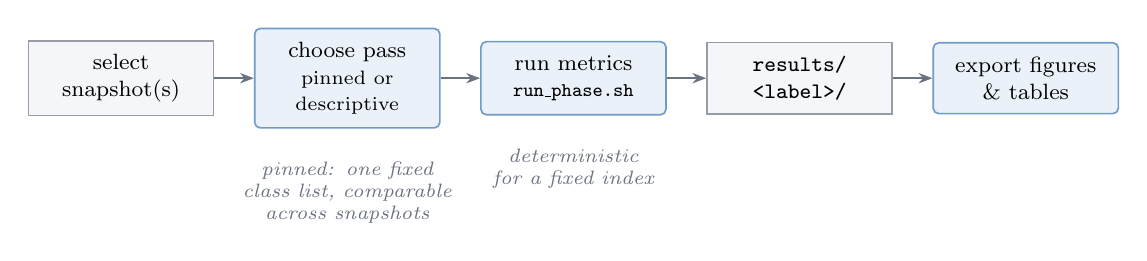
\begin{tikzpicture}[node distance=5mm,
    qbox/.style={stage, text width=20mm},
    qstore/.style={store, text width=20mm}]
  \node[qstore]            (sel)  {select\\snapshot(s)};
  \node[qbox, right=of sel](pass) {choose pass\\\scriptsize pinned or descriptive};
  \node[qbox, right=of pass](run) {run metrics\\\scriptsize\texttt{run\_phase.sh}};
  \node[qstore, right=of run](out){\texttt{results/}\\\texttt{<label>/}};
  \node[qbox, right=of out](read) {export figures\\\& tables};

  \draw[flow] (sel) -- (pass);
  \draw[flow] (pass) -- (run);
  \draw[flow] (run) -- (out);
  \draw[flow] (out) -- (read);

  \node[note, below=3mm of pass, text width=28mm]
       {pinned: one fixed class list, comparable across snapshots};
  \node[note, below=3mm of run, text width=24mm]
       {deterministic for a fixed index};
\end{tikzpicture}}

% ===========================================================================
% Dashboard screenshot slot. Renders the PNG when present, otherwise a marked
% placeholder of the same width, so the document always builds.
% ===========================================================================
\newcommand{\dashshot}[2]{%
  \IfFileExists{figures/#1}{\includegraphics[width=\linewidth]{figures/#1}}{%
    \fbox{\parbox[c][42mm][c]{.97\linewidth}{\centering\footnotesize
      \textcolor{kggrey}{screenshot placeholder}\\[2pt]
      \texttt{figures/#1}\\[4pt] #2}}}%
}
